%%%%%%%%%%%%%%%%%%%%%%%%%%%%%%%%%%%%%%%%%%%%%%
% Head matter - can we try to be consistent on
% included packages
\ifdefined\beamerclass
\else
    \def\beamerclass{beamer}
\fi
\documentclass[\beamerclass]{beamer}

\usepackage{pgfpages}
\mode<handout>{
	% \setbeamercolor{background canvas}{bg=black!20}
	\pgfpagesuselayout{2 on 1}[a4paper,border shrink=5mm]
}

%\documentclass{beamer}
\mode<presentation>
{\usetheme{default}
 \usecolortheme{default}
 \usefonttheme{default}
 \setbeamertemplate{navigation symbols}{}
 \setbeamertemplate{footline}[frame number]
% \setbeamertemplate{caption}[numbered]
 }
\usepackage[english]{babel}
\usepackage{algorithm}
\usepackage[noend]{algpseudocode}
\usepackage[utf8x]{inputenc}
\usepackage{graphicx}
\usepackage{hyperref}
%\graphicspath{{./images/}}
\usepackage{tikz}
\usetikzlibrary{shapes.geometric, arrows,chains}
\usepackage{booktabs,makecell,multirow,tabularx}
\usepackage{verbatim}
\renewcommand{\arraystretch}{1.2}
\renewcommand\theadfont{\normalfont\bfseries}
\usepackage{array}
\usepackage{listings}
\lstset{language=Java, showstringspaces=false}
\usepackage[normalem]{ulem}
\usepackage{bm}
\def\layersep{2.5cm}

\usepackage{xcolor}
%\usepackage{subfig}
\setbeamertemplate{caption}{\insertcaption}
\usepackage[caption=false]{subfig}
\usepackage{hyperref}
\usepackage{verbatim}
%\setbeamertemplate{caption}[numbered]%\numberwithin{figure}{section}
% Define block styles
\tikzstyle{decision} = [diamond, draw, fill=blue!20, 
    text width=4.5em, text badly centered, node distance=3cm, inner sep=0pt]
\tikzstyle{block} = [rectangle, draw, fill=blue!20, 
    text width=3em, text centered, rounded corners, minimum height=3em]
\tikzstyle{line} = [draw, -latex']
\tikzstyle{cloud} = [draw, ellipse, fill=red!20, node distance=3cm,
    minimum height=2em]
\tikzset{
  startstop/.style={
    rectangle, 
    rounded corners,
    minimum width=3cm, 
    minimum height=1cm,
    align=center, 
    draw=black, 
    fill=red!30
    },
  process/.style={
    rectangle, 
    minimum width=3cm, 
    minimum height=1cm, 
    align=center, 
    draw=black, 
    fill=blue!30
    },
  decision/.style={
    rectangle, 
    minimum width=3cm, 
    minimum height=1cm, align=center, 
    draw=black, 
    fill=green!30
    },
  arrow/.style={thick,->,>=stealth},
  dec/.style={
    ellipse, 
    align=center, 
    draw=black, 
    fill=green!30
    },
}
\tikzstyle{arrow} = [thick,->,>=stealth]

\tikzset{onslide/.code args={<#1>#2}{%
  \only<#1>{\pgfkeysalso{#2}} % \pgfkeysalso doesn't change the path
}}

\makeatletter
\newenvironment<>{btHighlight}[1][]
{\begin{onlyenv}#2\begingroup\tikzset{bt@Highlight@par/.style={#1}}\begin{lrbox}{\@tempboxa}}
{\end{lrbox}\bt@HL@box[bt@Highlight@par]{\@tempboxa}\endgroup\end{onlyenv}}

\newcommand<>\btHL[1][]{%
  \only#2{\begin{btHighlight}[#1]\bgroup\aftergroup\bt@HL@endenv}%
}
\def\bt@HL@endenv{%
  \end{btHighlight}%   
  \egroup
}
\newcommand{\bt@HL@box}[2][]{%
  \tikz[#1]{%
    \pgfpathrectangle{\pgfpoint{1pt}{0pt}}{\pgfpoint{\wd #2}{\ht #2}}%
    \pgfusepath{use as bounding box}%
    \node[anchor=base west, fill=orange!30,outer sep=0pt,inner xsep=1pt, inner ysep=0pt, rounded corners=3pt, minimum height=\ht\strutbox+1pt,#1]{\raisebox{1pt}{\strut}\strut\usebox{#2}};
  }%
}
\makeatother




%%%%%%%%%%%%%%%%%%%%%%%%%%%%%%%%%%%%%%%%%%%%%%
% Formatting for title page
\title[Deep Learning]{Going Deep}
\author{Kate Farrahi}
\institute{ECS Southampton}
\date{\today}
%%%%%%%%%%%%%%%%%%%%%%%%%%%%%%%%%%%%%%%%%%%%%%
\begin{document}
\begin{frame}
  \titlepage
\end{frame}
%%-------------------------------------------------------------%


%-------------------------------------------------------------%
%\begin{frame}[fragile]\frametitle{Deep Learning}
%Reading material \url{https://www.nature.com/articles/nature14539}
%\end{frame}
%-------------------------------------------------------------%
\begin{frame}{pause}\frametitle{The Universal Approximation Theorem} 

Let $\psi :\mathbb {R} \to \mathbb {R}$ be a nonconstant, bounded, and continuous function.  \pause
Let $ I_{m}$ denote the m-dimensional unit hypercube $[0,1]^m$. \pause
The space of real-valued continuous functions on $ I_{m}$ is denoted by $C(I_{m})$.  \pause 
Then, given any $\epsilon > 0$ and any function $f \in C(I_{m})$, there exist an integer $N$, real constants $v_i, b_i \in \mathbb{R} $ and real vectors $w_{i} \in \mathbb {R} ^{m}$ for $i=1,\ldots ,N$, such that we may define: \newline

$ F(x)=\sum _{i=1}^{N}v_{i} \psi (w_{i}^{T}x+b_{i}) $
as an approximate realization of the function $f$ ; that is, \pause \newline

$|F(x)-f(x)|<\epsilon $ \newline
for all  $x\in I_{m}$. 

%\url{https://www.youtube.com/watch?v=Ijqkc7OLenI}
%\url{https://www.youtube.com/watch?v=5dWp1mw_XNk&index=40&list=PLkDaE6sCZn6Ec-XTbcX1uRg2_u4xOEky0}
\end{frame}
%-------------------------------------------------------------%

\begin{frame}{pause}\frametitle{Then Why Go Deep?} 
\begin{itemize}
\item There are functions you can compute with a deep neural network that shallow networks require exponentially more hidden units to compute.
\item The following function is more efficient to implement using a deep neural network: $y = x_1 \oplus x_2 \oplus x_3 \oplus \dots \oplus x_n$
\end{itemize}
\end{frame}
%-------------------------------------------------------------%

\begin{frame}{pause}\frametitle{Vanishing and Exploding Gradients}
\begin{itemize}
\item The vanishing and exploding gradient problem is a difficulty found in training NN with gradient-based learning methods and backpropagation.  \pause
\item In training, the gradient may become vanishingly small (or large), effectively preventing the weight from changing its value (or exploding in value). \pause
\item This leads to the neural network not being able to train. \pause
\item This issue affects many-layered networks (feed-forward), as well as recurrent networks. 
\end{itemize}
\end{frame}
%-------------------------------------------------------------%

\begin{frame}{pause}\frametitle{Issues with Going Deep}
\centering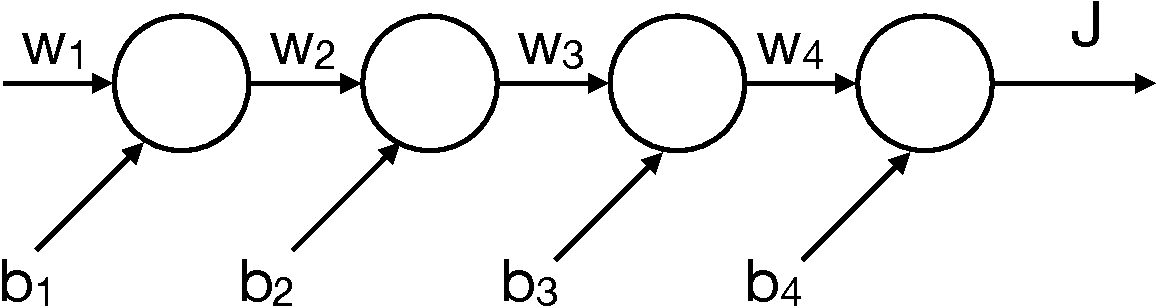
\includegraphics[width=10cm]{deep.pdf}
\end{frame}
%-------------------------------------------------------------%

\begin{frame}{pause}\frametitle{Residual Connections}

\begin{itemize}
\item One of the most effective ways to resolve the vanishing gradient problem is with residual neural networks (ResNets)\footnote{K. He, X. Zhang, S. Ren and J. Sun, "Deep Residual Learning for Image Recognition," CVPR, Las Vegas, NV, 2016, pp. 770-778.}. \pause
\item ResNets are artificial neural networks that use {\em skip connections} to jump over  layers. \pause
\item The vanishing gradient problem is mitigated in ResNets by reusing activations from a previous layer. 
\end{itemize}
\end{frame}
%-------------------------------------------------------------%

\begin{frame}{pause}\frametitle{Residual Connections}

\centering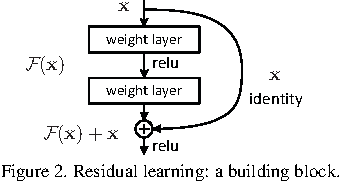
\includegraphics{ResBlock.pdf} \footnote{K. He, X. Zhang, S. Ren and J. Sun, "Deep Residual Learning for Image Recognition," CVPR, Las Vegas, NV, 2016, pp. 770-778.}.
\end{frame}
%-------------------------------------------------------------%

\begin{frame}{pause}\frametitle{Residual Connections}
\centering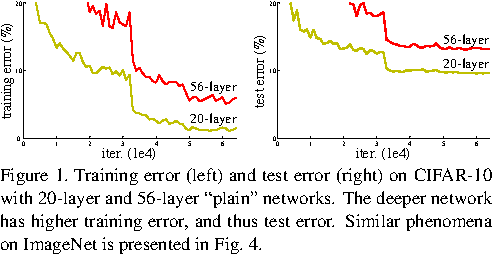
\includegraphics[width=10cm]{Fig1.pdf}\footnote{K. He, X. Zhang, S. Ren and J. Sun, "Deep Residual Learning for Image Recognition," CVPR, Las Vegas, NV, 2016, pp. 770-778.}
\end{frame}
%-------------------------------------------------------------%

\begin{frame}{pause}\frametitle{Residual Connections}
\centering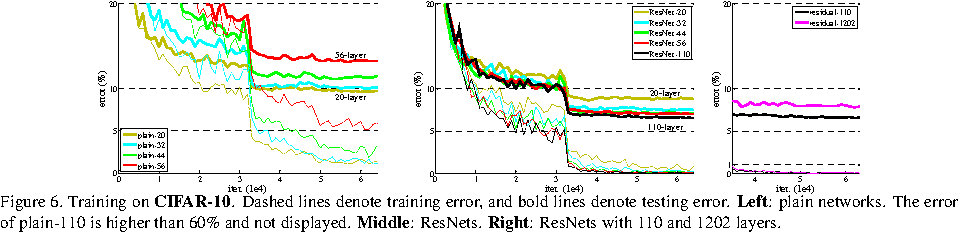
\includegraphics[width=11cm]{Fig6.pdf}\footnote{K. He, X. Zhang, S. Ren and J. Sun, "Deep Residual Learning for Image Recognition," CVPR, Las Vegas, NV, 2016, pp. 770-778.}
\end{frame}
%-------------------------------------------------------------%

\begin{frame}{pause}\frametitle{Dropout}
\begin{itemize}
\item Neural networks with a large number of parameters (and hidden layers) are powerful, however, overfitting is a serious problem in such systems. \pause
\item Dropout is a form of regularization \pause
\item The key idea in dropout is to randomly drop neurons, including all of the connections, from the neural network during training.
\end{itemize}
\end{frame}
%-------------------------------------------------------------%
\begin{frame}[fragile]\frametitle{Dropout}
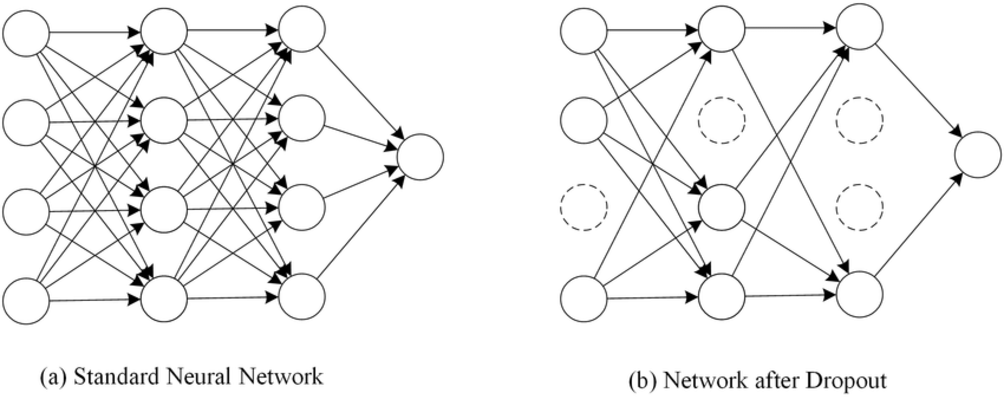
\includegraphics[width=10cm]{dropout.pdf} \footnote{Image from: \url{https://www.researchgate.net/figure/Dropout-neural-network-model-a-is-a-standard-neural-network-b-is-the-same-network_fig3_309206911}}
\end{frame}
%-------------------------------------------------------------%
\begin{frame}{pause}\frametitle{How Does Dropout Work in Practice?}
\begin{itemize}
\item In the learning phase, we stochastically remove hidden units by setting a dropout probability for each layer in the network. We then randomly decide wether or not a neuron in a given layer is removed stochastically. 
\end{itemize}
\end{frame}
%-------------------------------------------------------------%
\begin{frame}{pause}\frametitle{How Does Dropout Work in Practice?}
\begin{itemize}
\item We define a random binary mask $m^{(l)}$ which is used to remove neurons, and note, $m^{(l)}$ changes for each iteration of the backpropagation algorithm. \pause
\item For layers, $l = 1$  to  $L-1$, for the forward pass of backpropagation, we then compute 
\begin{equation}
a^{(l)} = \sigma(w^{(l)} a^{(l - 1)} + b^{(l)})  \odot m^{(l)}
\end{equation} \pause
\item For layer $L$, 
\begin{equation}
a^{(L)} = \sigma(w^{(L)} a^{(L - 1)} + b^{(l)})
\end{equation} \pause
\item For the backward pass of the backpropagation algorithm, 
\begin{equation} \delta^L = \Delta_a J \odot \sigma^{\prime} (z^L) \end{equation} \pause
\begin{equation} \delta^l = ((w^{l + 1})^T \delta^{l + 1}) \odot \sigma^{\prime} (z^l) \odot m^{(l)} \end{equation} 
\end{itemize}
\end{frame}
%-------------------------------------------------------------%

\begin{frame}{pause}\frametitle{Why Does Dropout Work?}
\begin{itemize}
\item Neurons cannot co-adapt to other units (they cannot assume that all of the other units will be present) \pause
\item By breaking co-adaptation, each unit will ultimately find more general features
\end{itemize}
\end{frame}
%-------------------------------------------------------------%
%\begin{frame}{pause}\frametitle{Batch Norm}
%\begin{itemize}
%\item Batch Normalization allows us to use much higher learning rates and be less careful about initialization.  \pause
%\item It also acts as a regularizer, in some cases eliminating the need for Dropout. 
%\end{itemize}
%\end{frame}
%-------------------------------------------------------------%

\end{document}
